
\chapter{任务需求分析}

在本次实验中,我们完成了一个完整的 HTTP 服务器。能够处理\textbf{并发的},\textbf{大量的}符合\textbf{HTTP 1.1}的请求报文,并且能够支持对\textbf{CGI}请求做特殊处理。以下将分别介绍四周、以及选做的任务需求及分析。

\section{第一周:实现简单的 echo web server} 第一关的任务主要分为以下几点:
\begin{enumerate}
    \item 搭建编程环境、熟悉 Socket 编程方法,为之后的任务奠定基础;
    \item 完成消息解析模块,为服务器实现基本的功能做好准备;
    \item 完成基本的错误码返回以及基础方法 HEAD、GET、POST 的判断,为以后分别处理不同的报文,同时测试模块化、解耦和的编程框架;
\end{enumerate}
    

总地来看,第一周任务的主要目的,是让我们熟悉编程环境以及 socket 的基础功能。万事开头难,完成第一关的任务,将对我们完成剩下的任务奠定一个良好、坚实的基础。

\section{第二周:实现 HEAD、GET、POST 方法} 第二关的任务主要为以下几点:
\begin{enumerate}
    \item 完善服务器的功能、能够建立并维系 HEAD、GET、POST 的持久连接;(此时还不需要进行 Pipelining)
    \item 支持 4 种 HTTP 1.1 错误码、能够正确封装响应消息;
    \item 妥善管理缓冲区、避免客户端请求消息过长导致缓冲区溢出,该项任务\textbf{主要目的}在于处理 1. 下一步 Pipelining 请求过长,以及 2. 后续 CGI 处理 POST 请求时,可能会有大量参数传递,导致溢出的情况;
    \item 处理读写磁盘错误,防止因为错误导致服务器宕机等问题;
    \item 进行格式化日志的记录,方便正式上线后的 Debug;
\end{enumerate}

第二周的任务是对于 server 处理框架的优化,引导我们去实现独立的消息处理和日志模块等,解耦和、模块化的编程框架为之后的编程提供了便利和良好的可扩展性。

\section{第三周:实现 HTTP 并发请求} 第三关的任务主要为:
\begin{enumerate}
    \item 服务器能够连续相应客户端的 Pipelining 请求; 
    \item 即使出现了错误的请求,也妨碍服务器进行剩下并发请求的处理;
\end{enumerate}

第三周的任务是对于 server 端的能力进行提升,作为一个比较单独的功能,是根据 RFC2616 文档标准设计出来的并发请求模式。是我们实现标准 HTTP 服务器的关键之处。

\section{第四周:实现多个客户端的并发处理} 第四关的任务主要是:
\begin{enumerate}
    \item 使用 select 函数实现多用户并发请求,在其他用户暂停发送时,服务器能察觉并转而给其他用户提供服务;
    \item 服务器的最大连接数量设置为 1024,为 Linux 最大的文件描述符;
\end{enumerate}

第四周的任务是 HTTP 1.1 中较为独立且较为困难的协议之一。在理论上来说,我们只需要在第三周止步即可实现一个完整的服务端程序。然而第四周的 select 为多用户并发的情况进行了非常好的优化,是向市面上的服务端靠齐的一个关键。在这一关中,我们还将使用 apache bench 对服务器性能进行评测,这也是向正规服务器看齐的关键。

\section{选做:CGI}
\begin{enumerate}
    \item 根据 RFC3875 以及 RFC2396 文档,实现 CGI 的请求;
    \item CGI 请求的处理主要靠 URI 区别,且将用一个新的线程处理该请求;
\end{enumerate}

该任务的完成,将标志着我们的服务器走向新的一个台阶:它将能够正确处理 POST 请求,且拥有作为后端程序与前端界面进行交互的能力。当然,对于 session 等更高级的网络编程工具的支持,尚未开发。至少通过我们的实现,我们将能够实现一个非常基础的用户注册、登陆接口。

由于我们将采用 Python - 数据库的技术栈,所以我们能够对用户信息进行记录,同时方便对以后想添加的其他功能进行扩展。

如图 \ref{fig:cgi1} 我们在自己的阿里云服务器上部署项目,方便测试与演示。

\begin{figure}[htbp!]
    \centering
    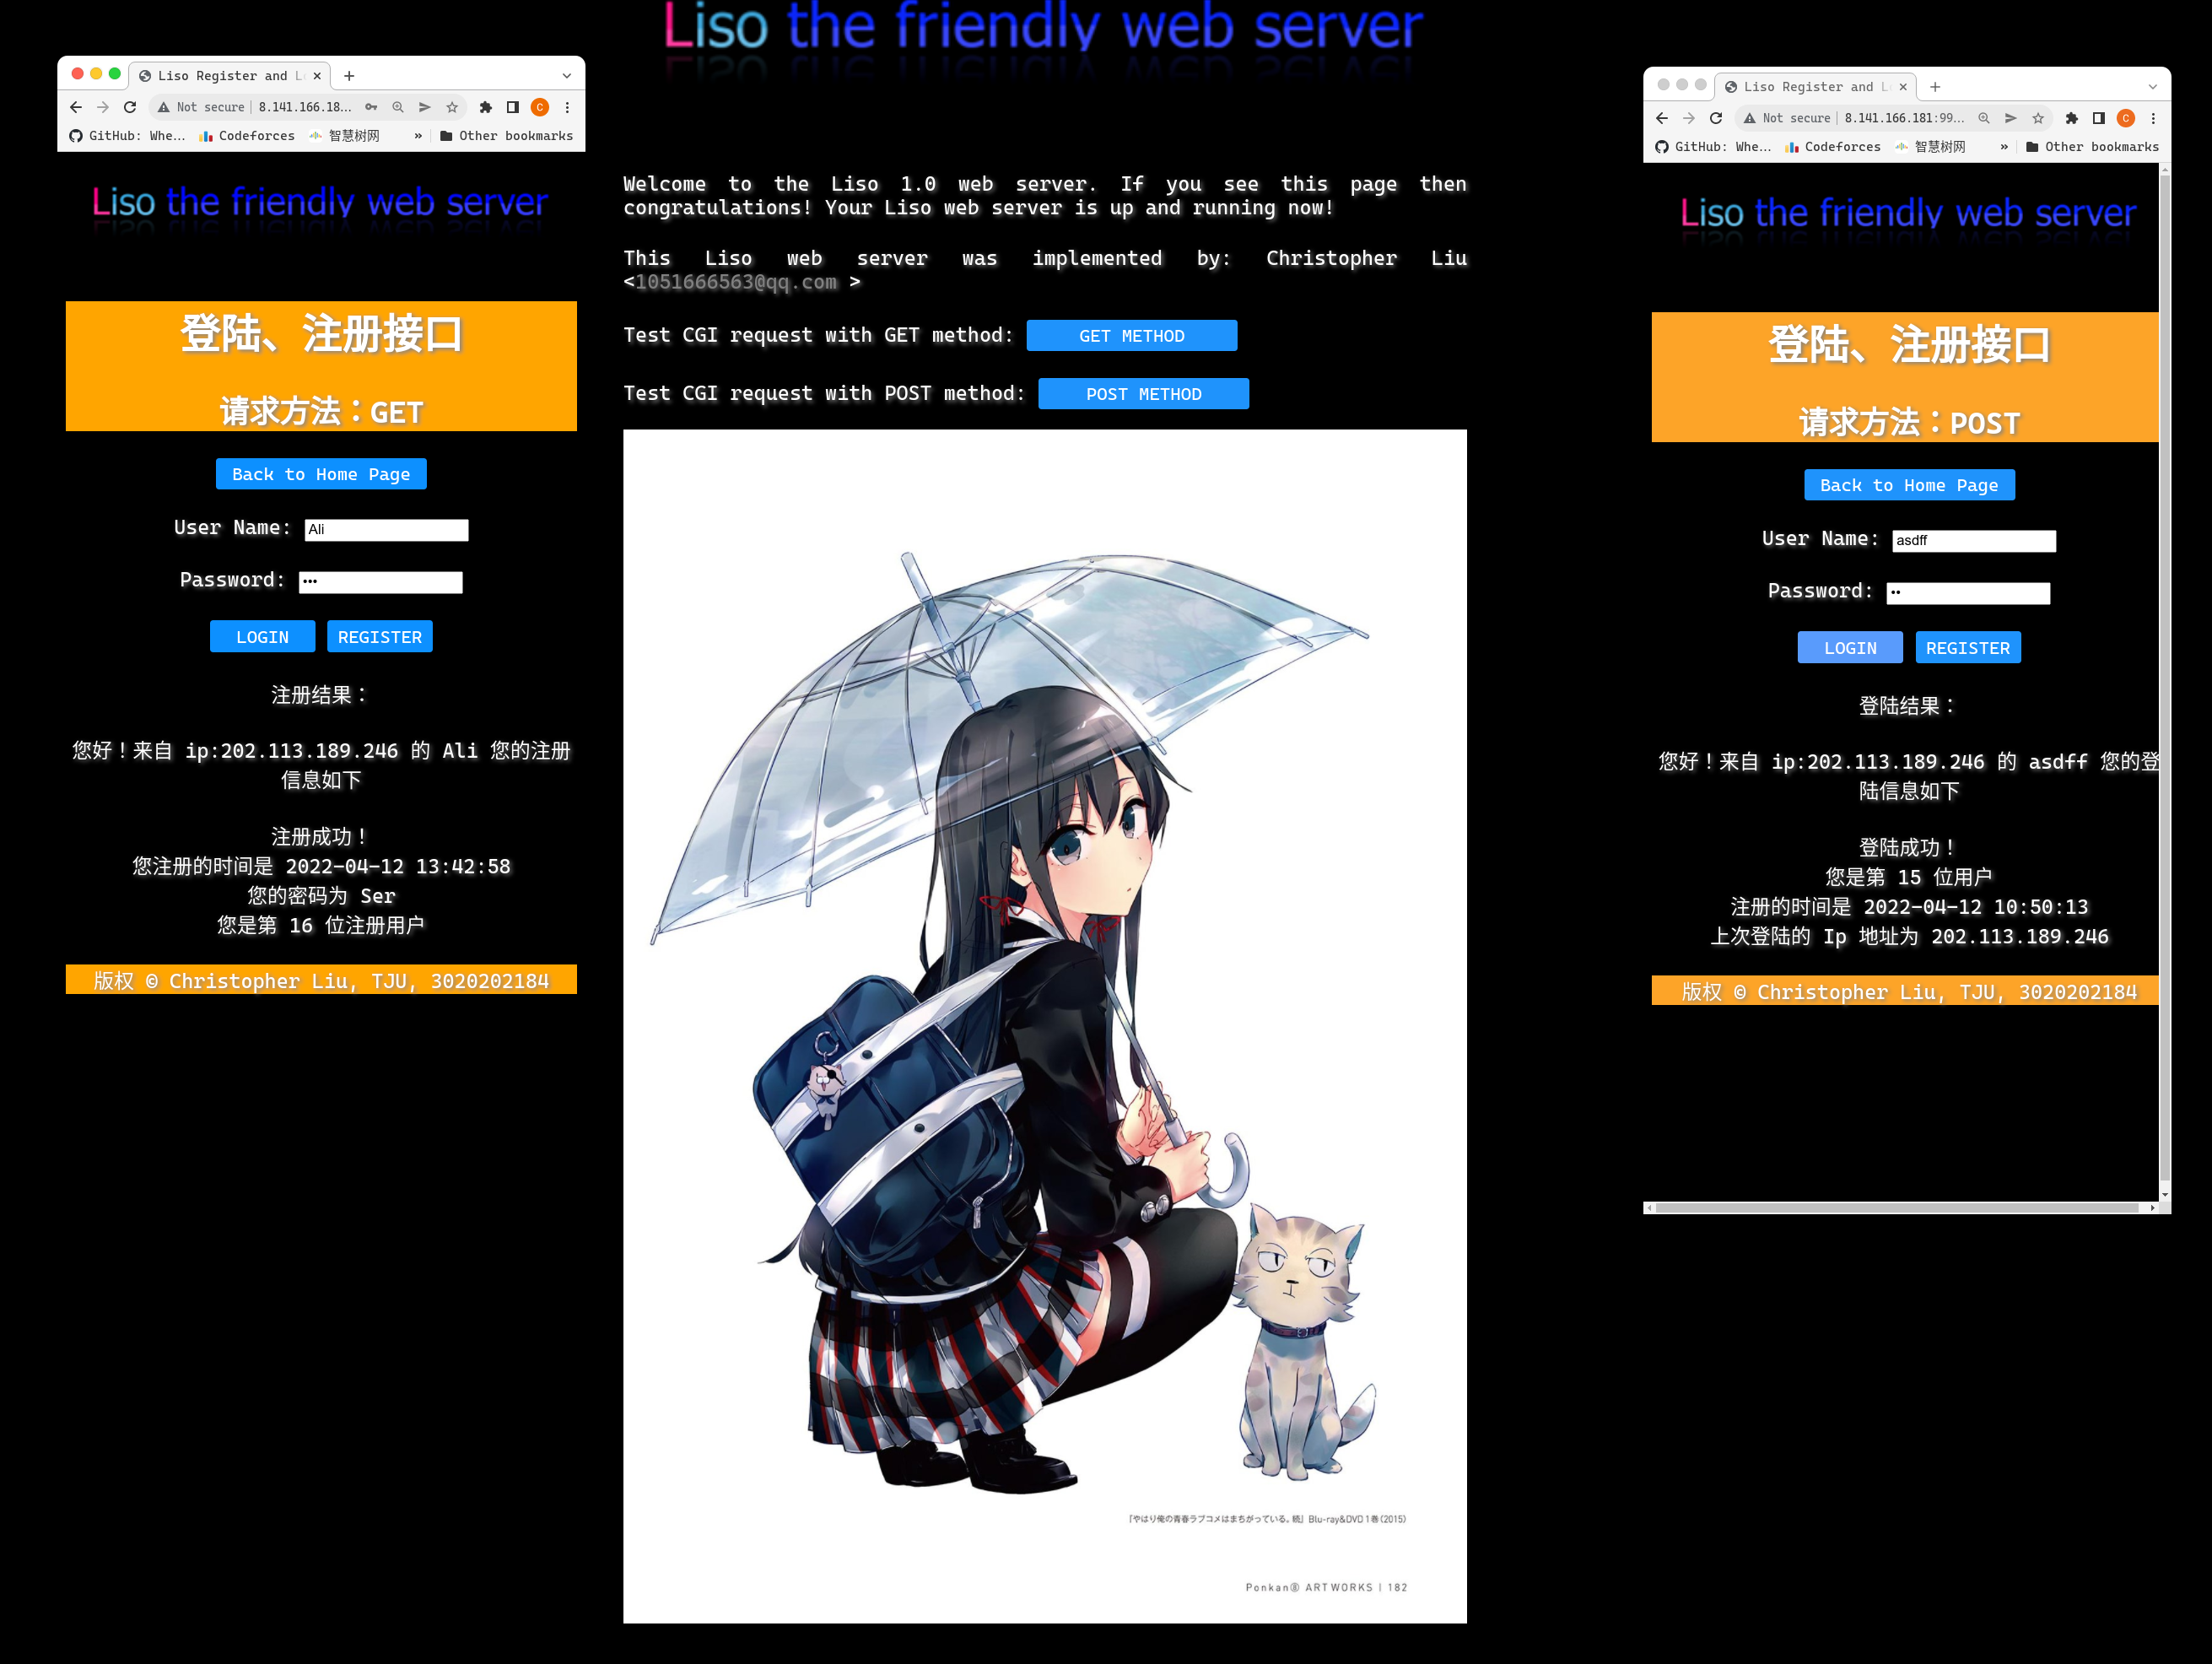
\includegraphics[width=3.3in]{Liso_Complete.png}
    \caption{CGI 成品样例}\label{fig:cgi1}
\end{figure}




